\begin{figure*}
  \centering
  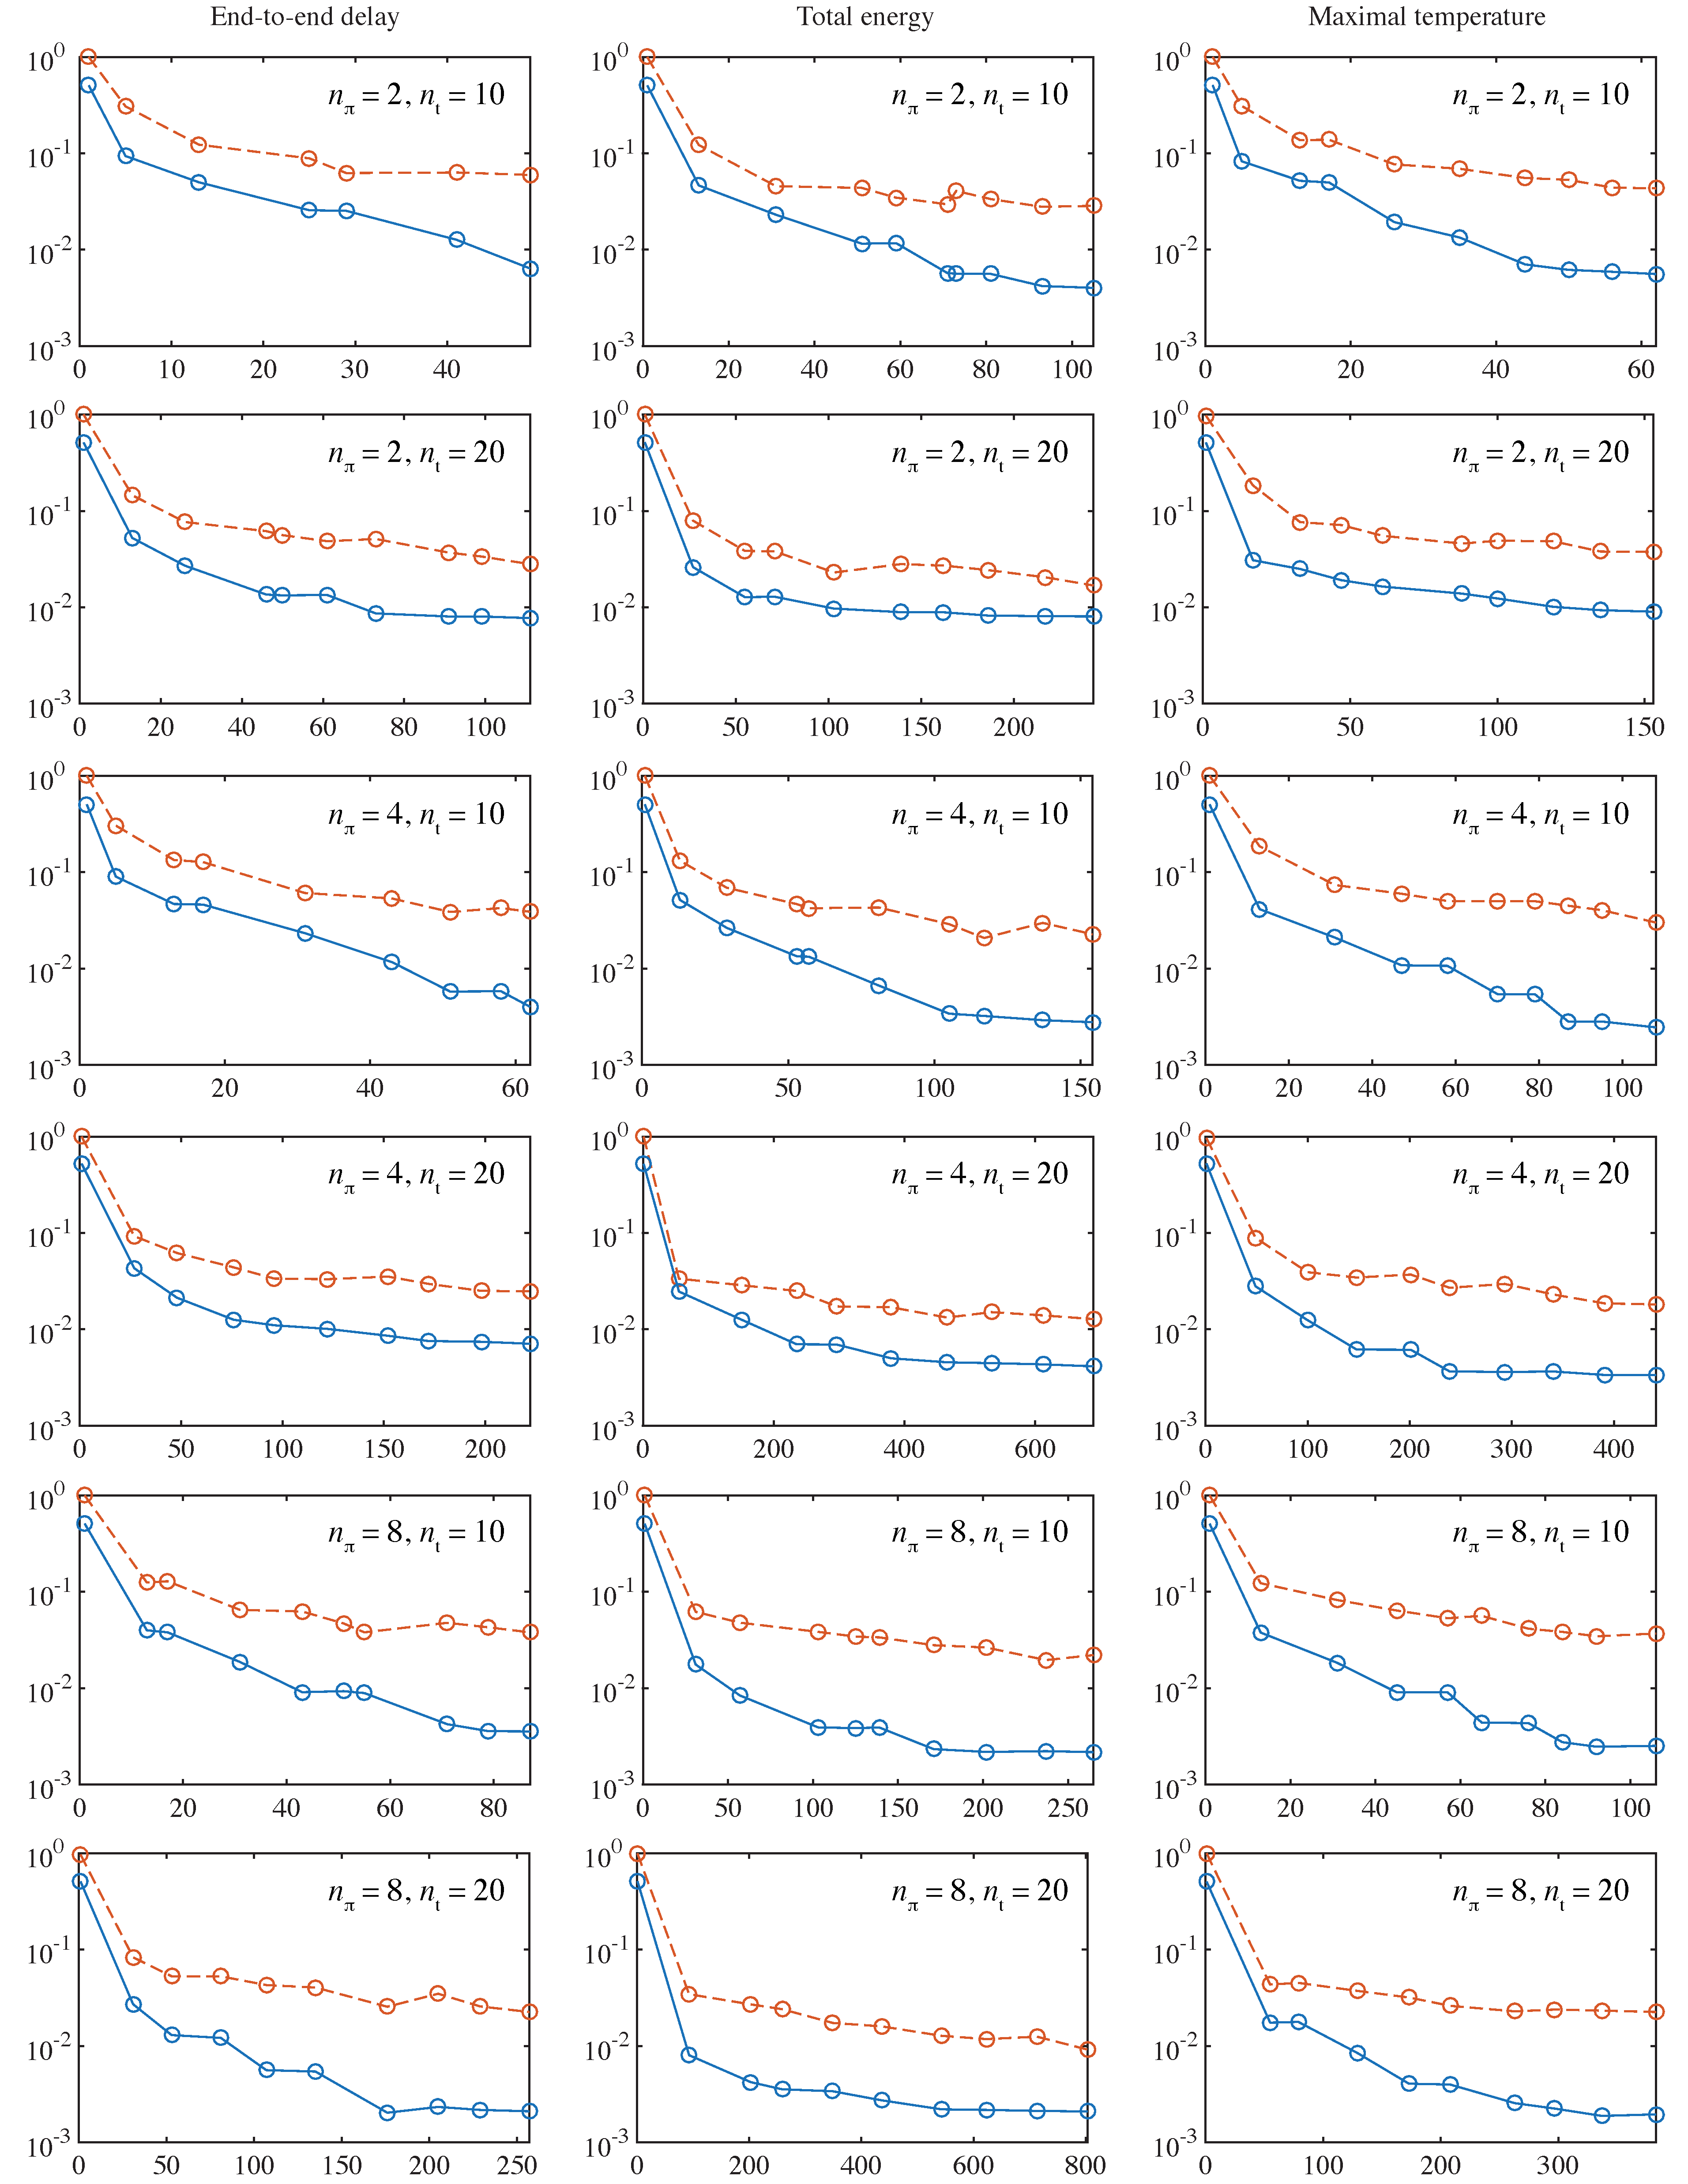
\includegraphics[width=1.0\textwidth]{include/assets/figures/results.pdf}
  \hspace{-1em}
  \caption{
    Experimental results. There are considered 3 quantities of interest, 3
    platform sizes, and 2 application sizes, which results in 18 problems in
    total. The columns correspond to the three quantities of interest: the
    end-to-end delay (left), total energy (middle), and maximum temperature
    (right). The three pairs of rows correspond to the three platform sizes: 2
    (top), 4 (middle), and 8 (bottom) processing elements. The rows alternate
    between the two application sizes: 10 (odd) and 20 (even) tasks. The
    horizontal axes show the number of points. The vertical axes show the error
    on a logarithmic scale.
  }
  \flab{results}
\end{figure*}
